% -*- TeX-master: "YFT2023.tex"; eval: (longlines-mode); fill-column: 100000 -*-

\newpage

\section{Appendices}
\label{sec:appendices}

\renewcommand\thefigure{\thesection.\arabic{figure}}
\renewcommand\thetable{\thesection.\arabic{table}}

\subsection{Likelihood profiles}
\label{sec:likelihood_profile}

The approach for calculating a likelihood profile of the total population scaling parameter is outlined in \autoref{sec:parameter_uncertainty}. The profile reflects the loss of fit over all the data, i.e., the overall objective function value, caused by changing the population scale from that of the maximum likelihood estimated value. A range of fixed values were used until the best fit for each data source was found. The likelihood profile for the diagnostic model is shown in \autoref{fig:likelihood_profile} for narrow and wide widows around the maximum likelihood estimated value.

Likelihood profiles on the total population scaling parameter are also included for individual fisheries length and weight compositions to explore sources of conflict in these data, \autoref{fig:likelihood_profile_weight} and \autoref{fig:likelihood_profile_length}.

\setcounter{figure}{0}
\begin{figure}[H]
  \centering
  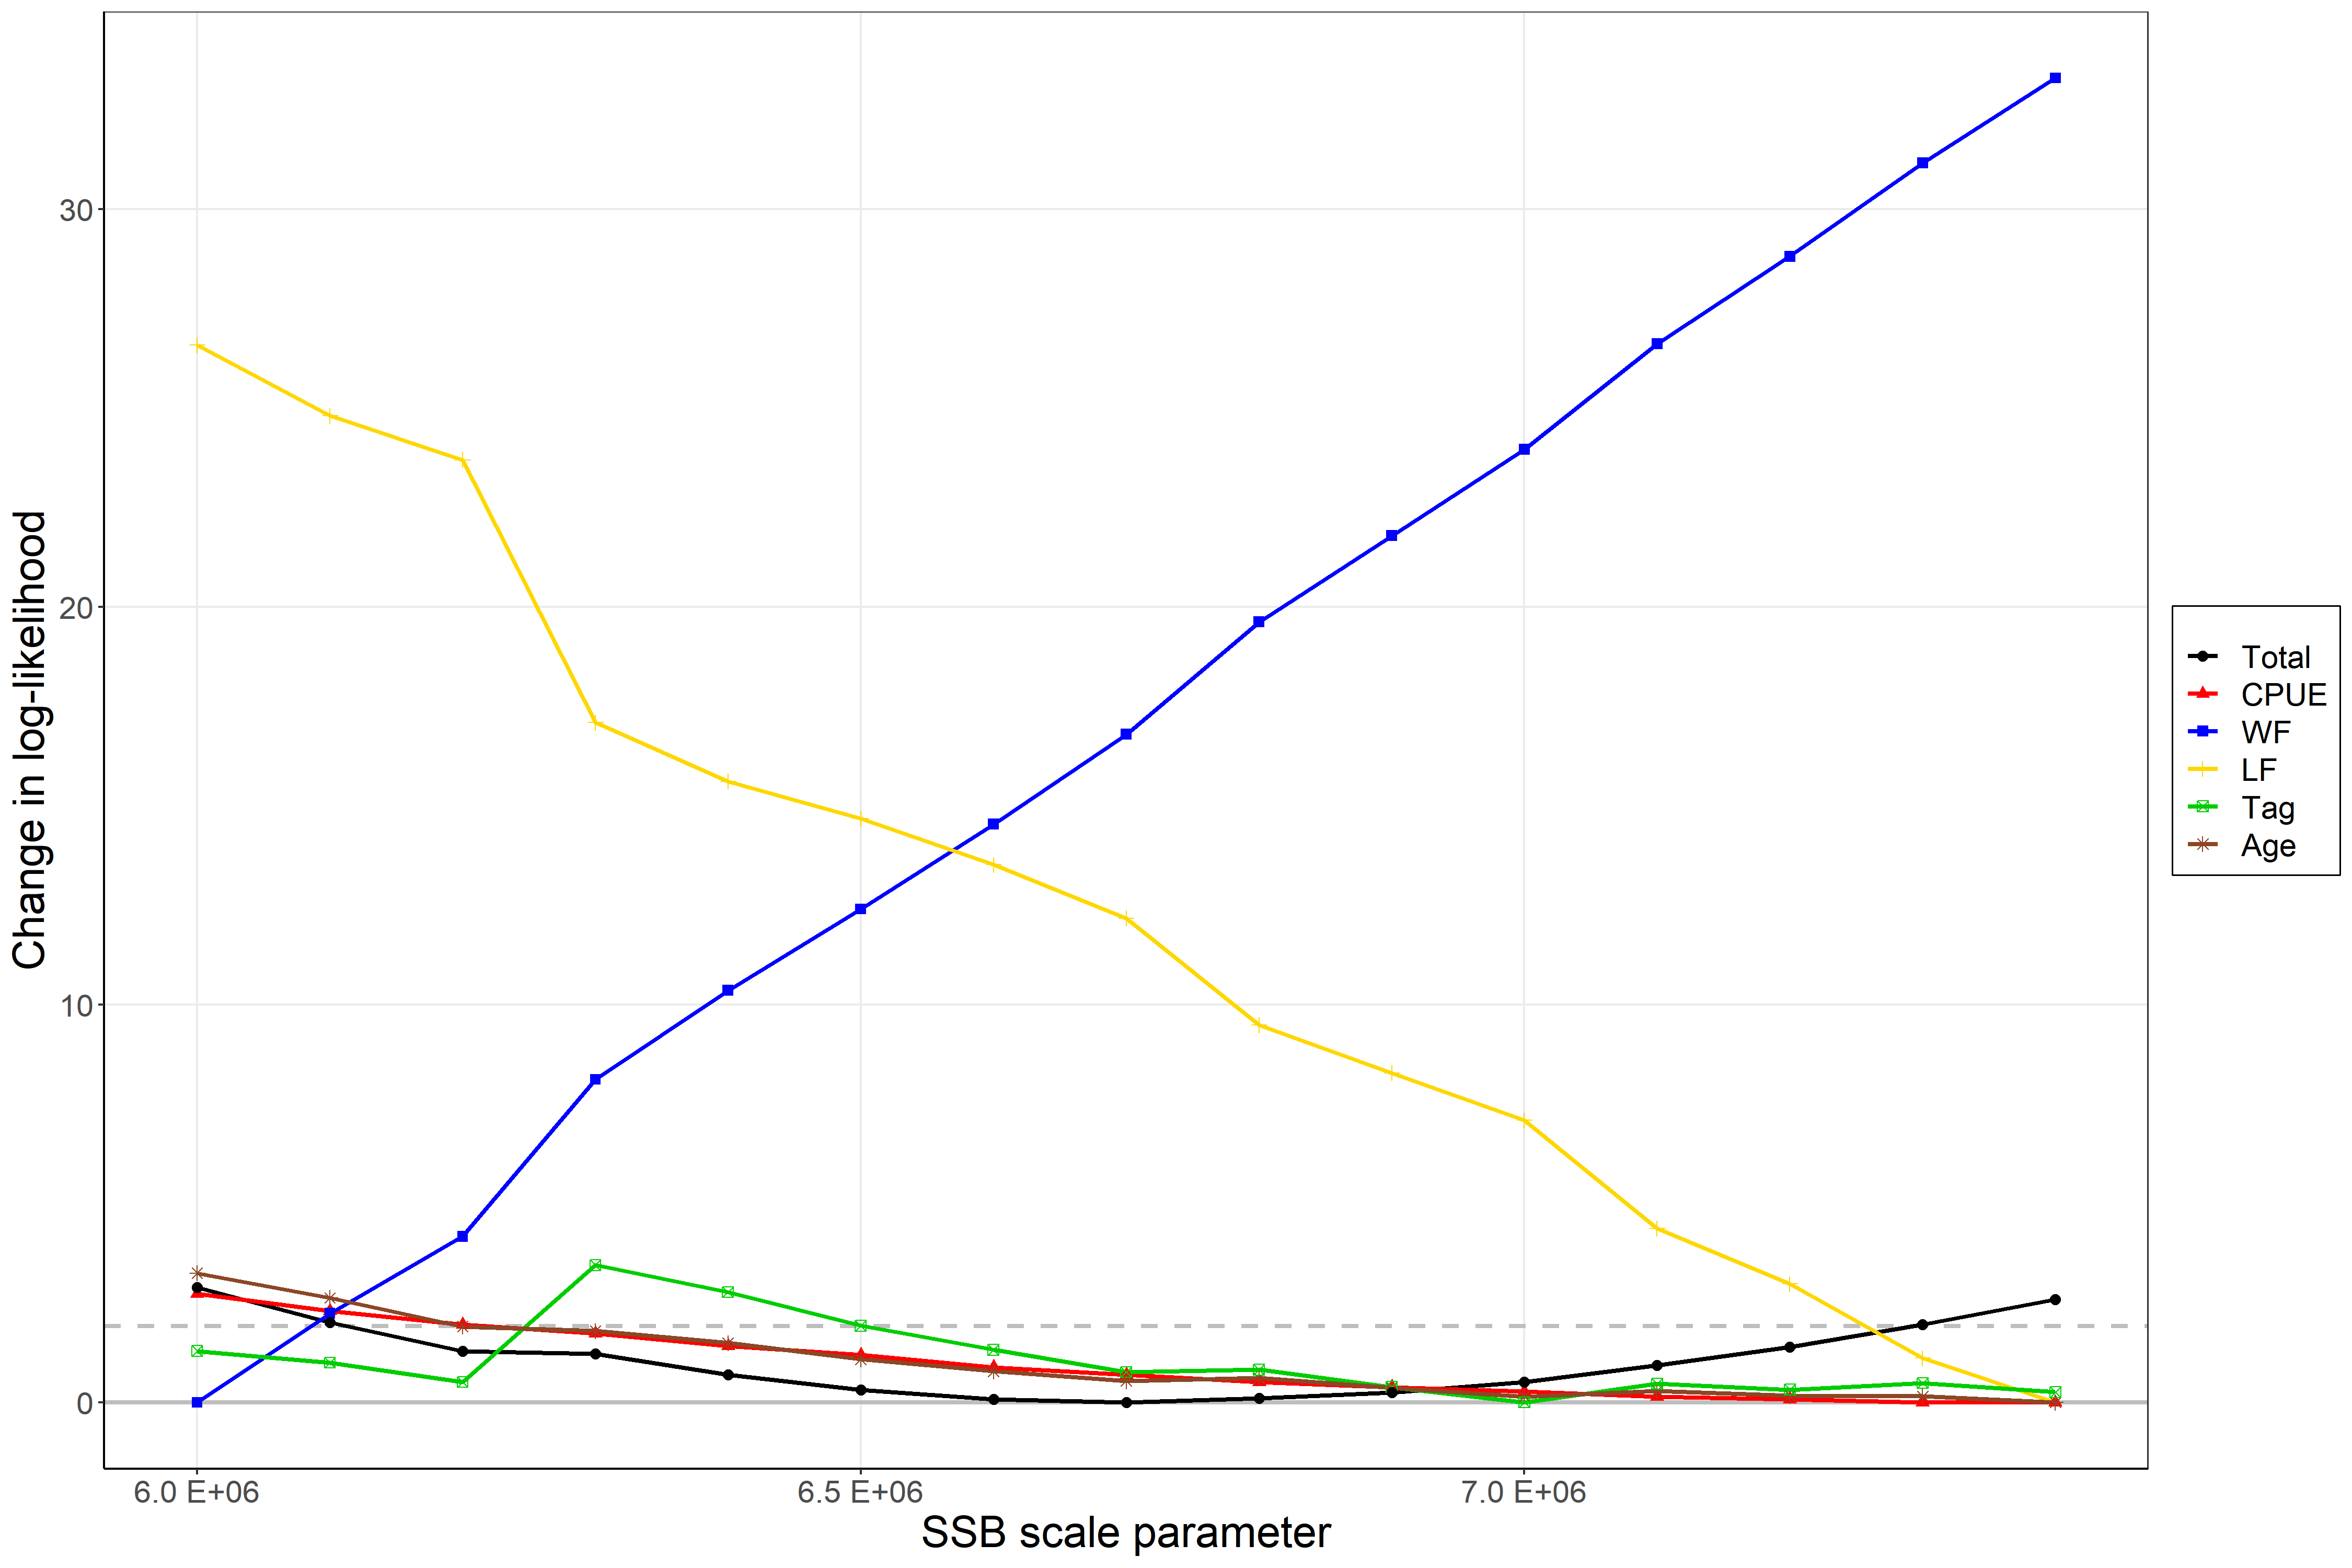
\includegraphics[width=0.8\textwidth]{likelihoodprofile_narrow.png}\\[10mm]
  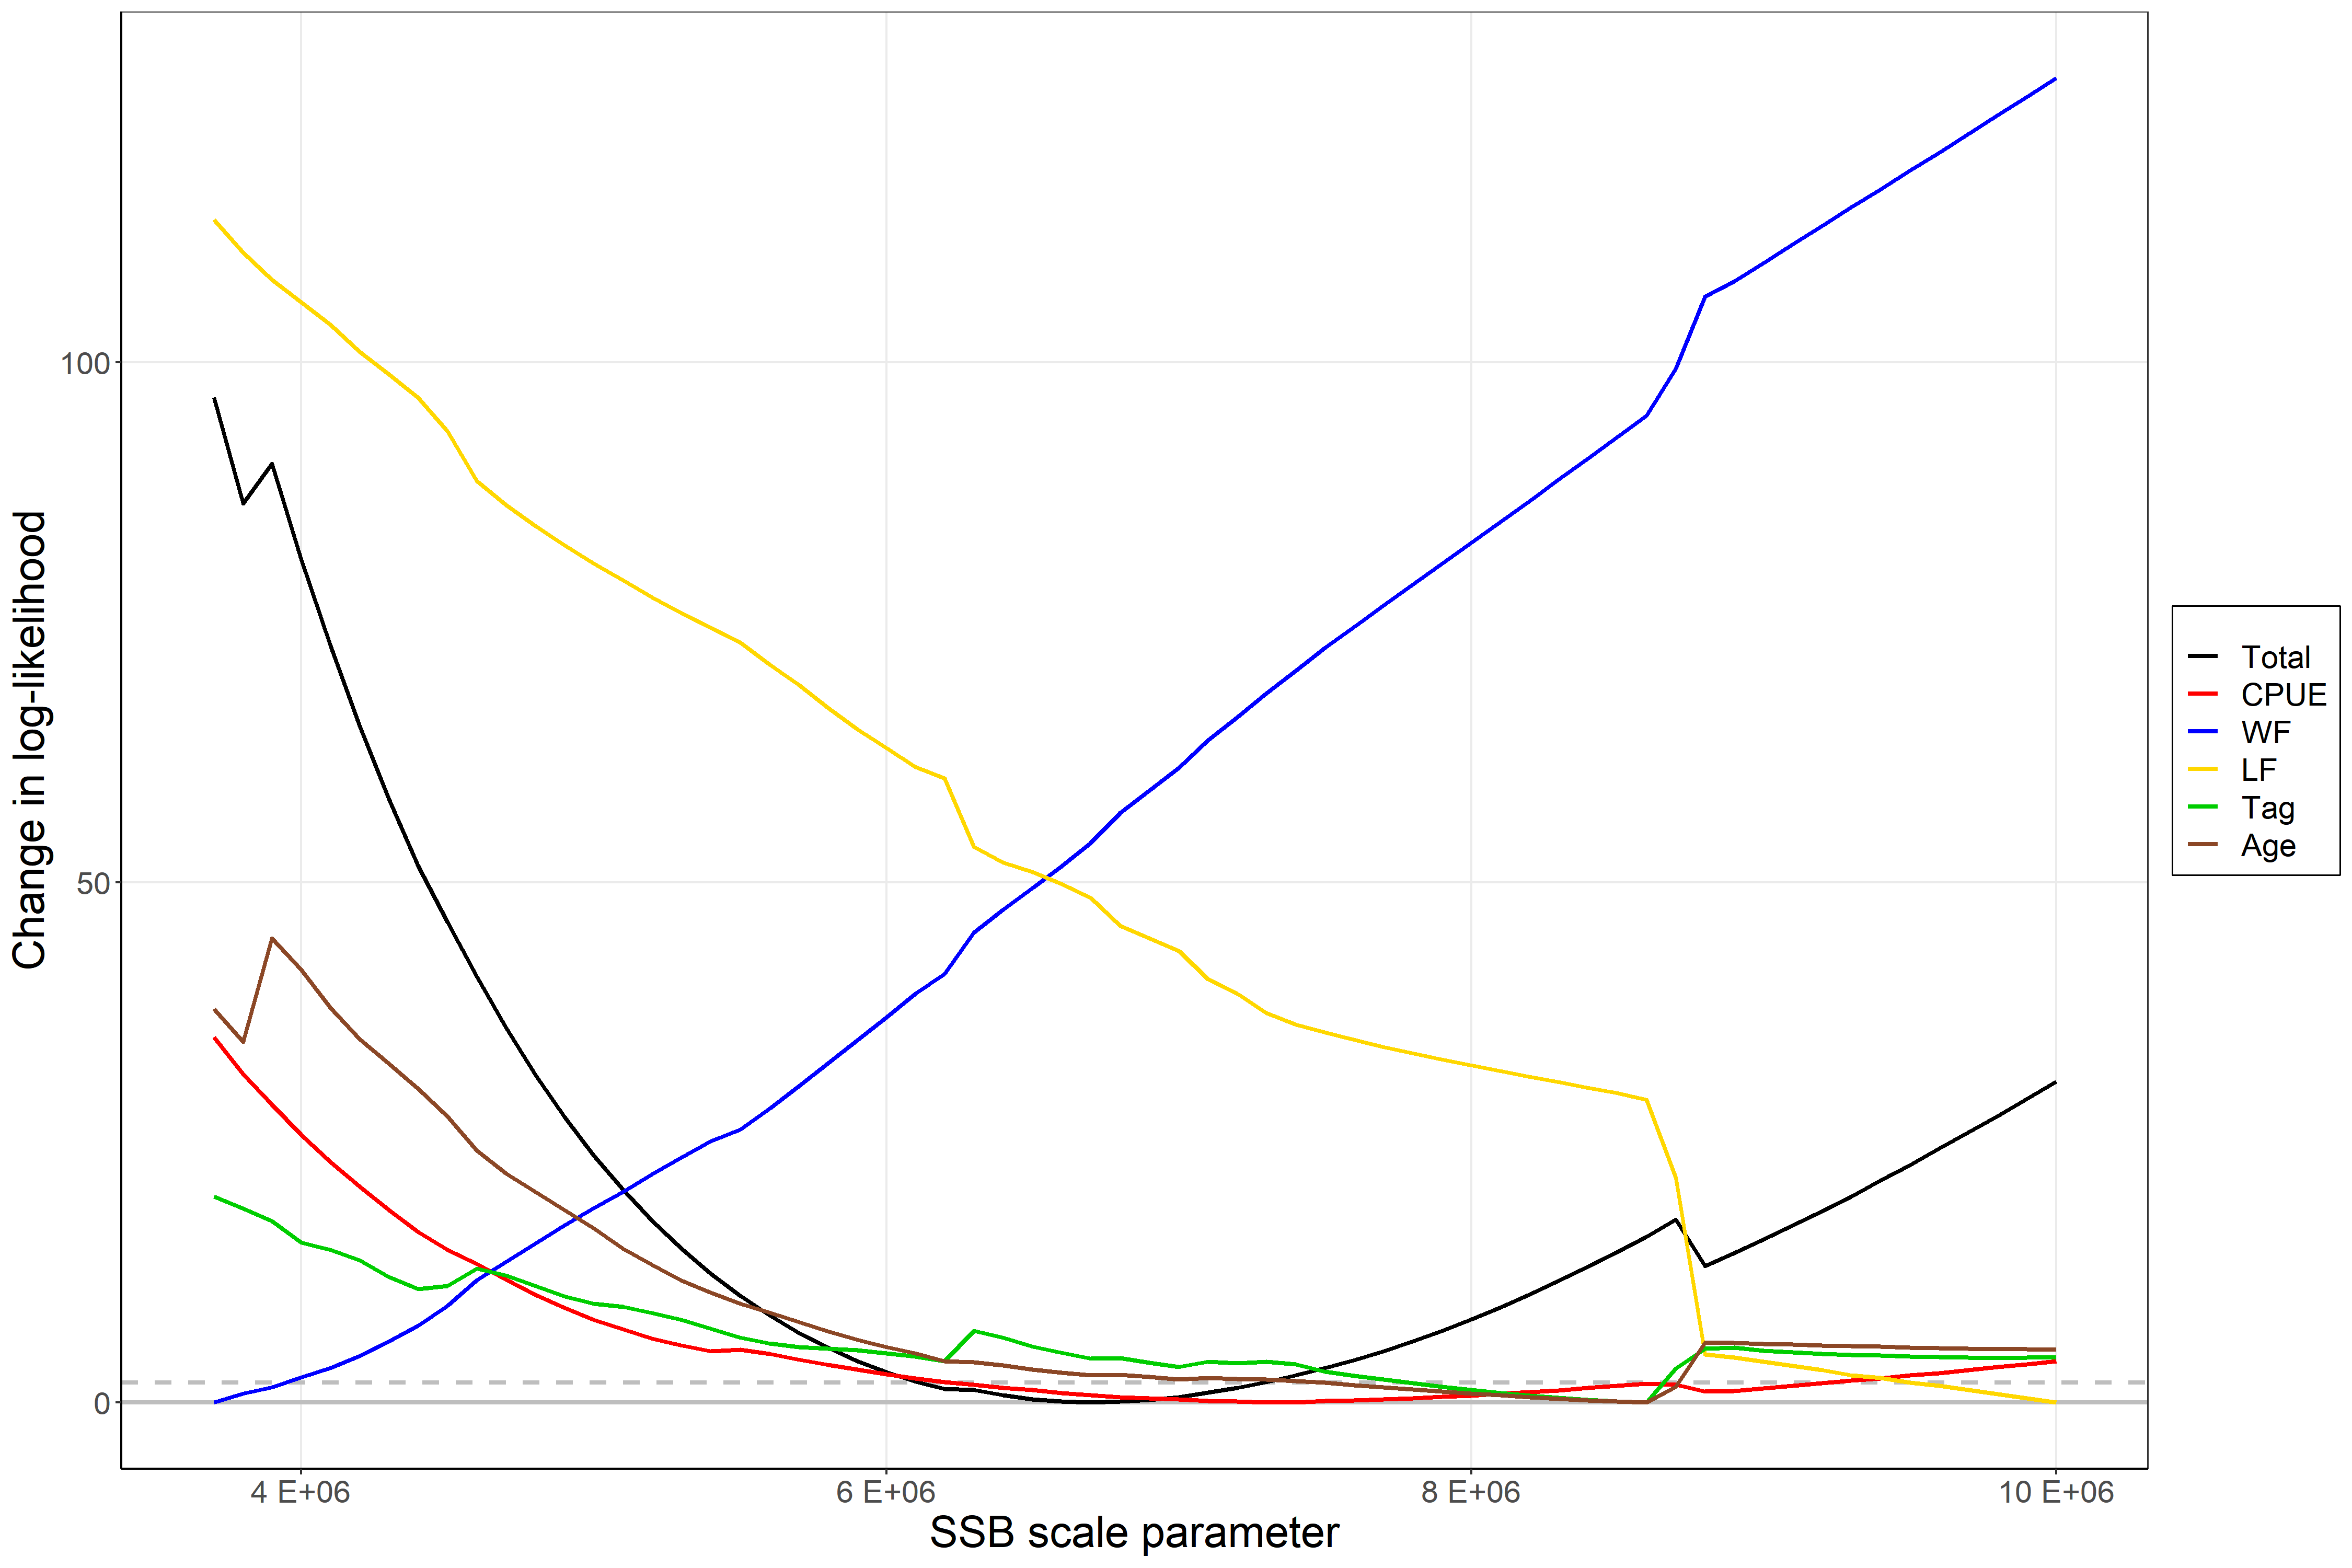
\includegraphics[width=0.8\textwidth]{likelihoodprofile_wide.png}
  \caption{Profiles of the total log-likelihood with respect to average total biomass in million mt across a range of fixed values for the model data sources, the black line indicates the total likelihood. The top plot shows a narrow window around the maximum likelihood estimated value and the bottom plot shows a wider window. \label{fig:likelihood_profile}}
\end{figure}

\clearpage

\begin{figure}[H]
  \centering
  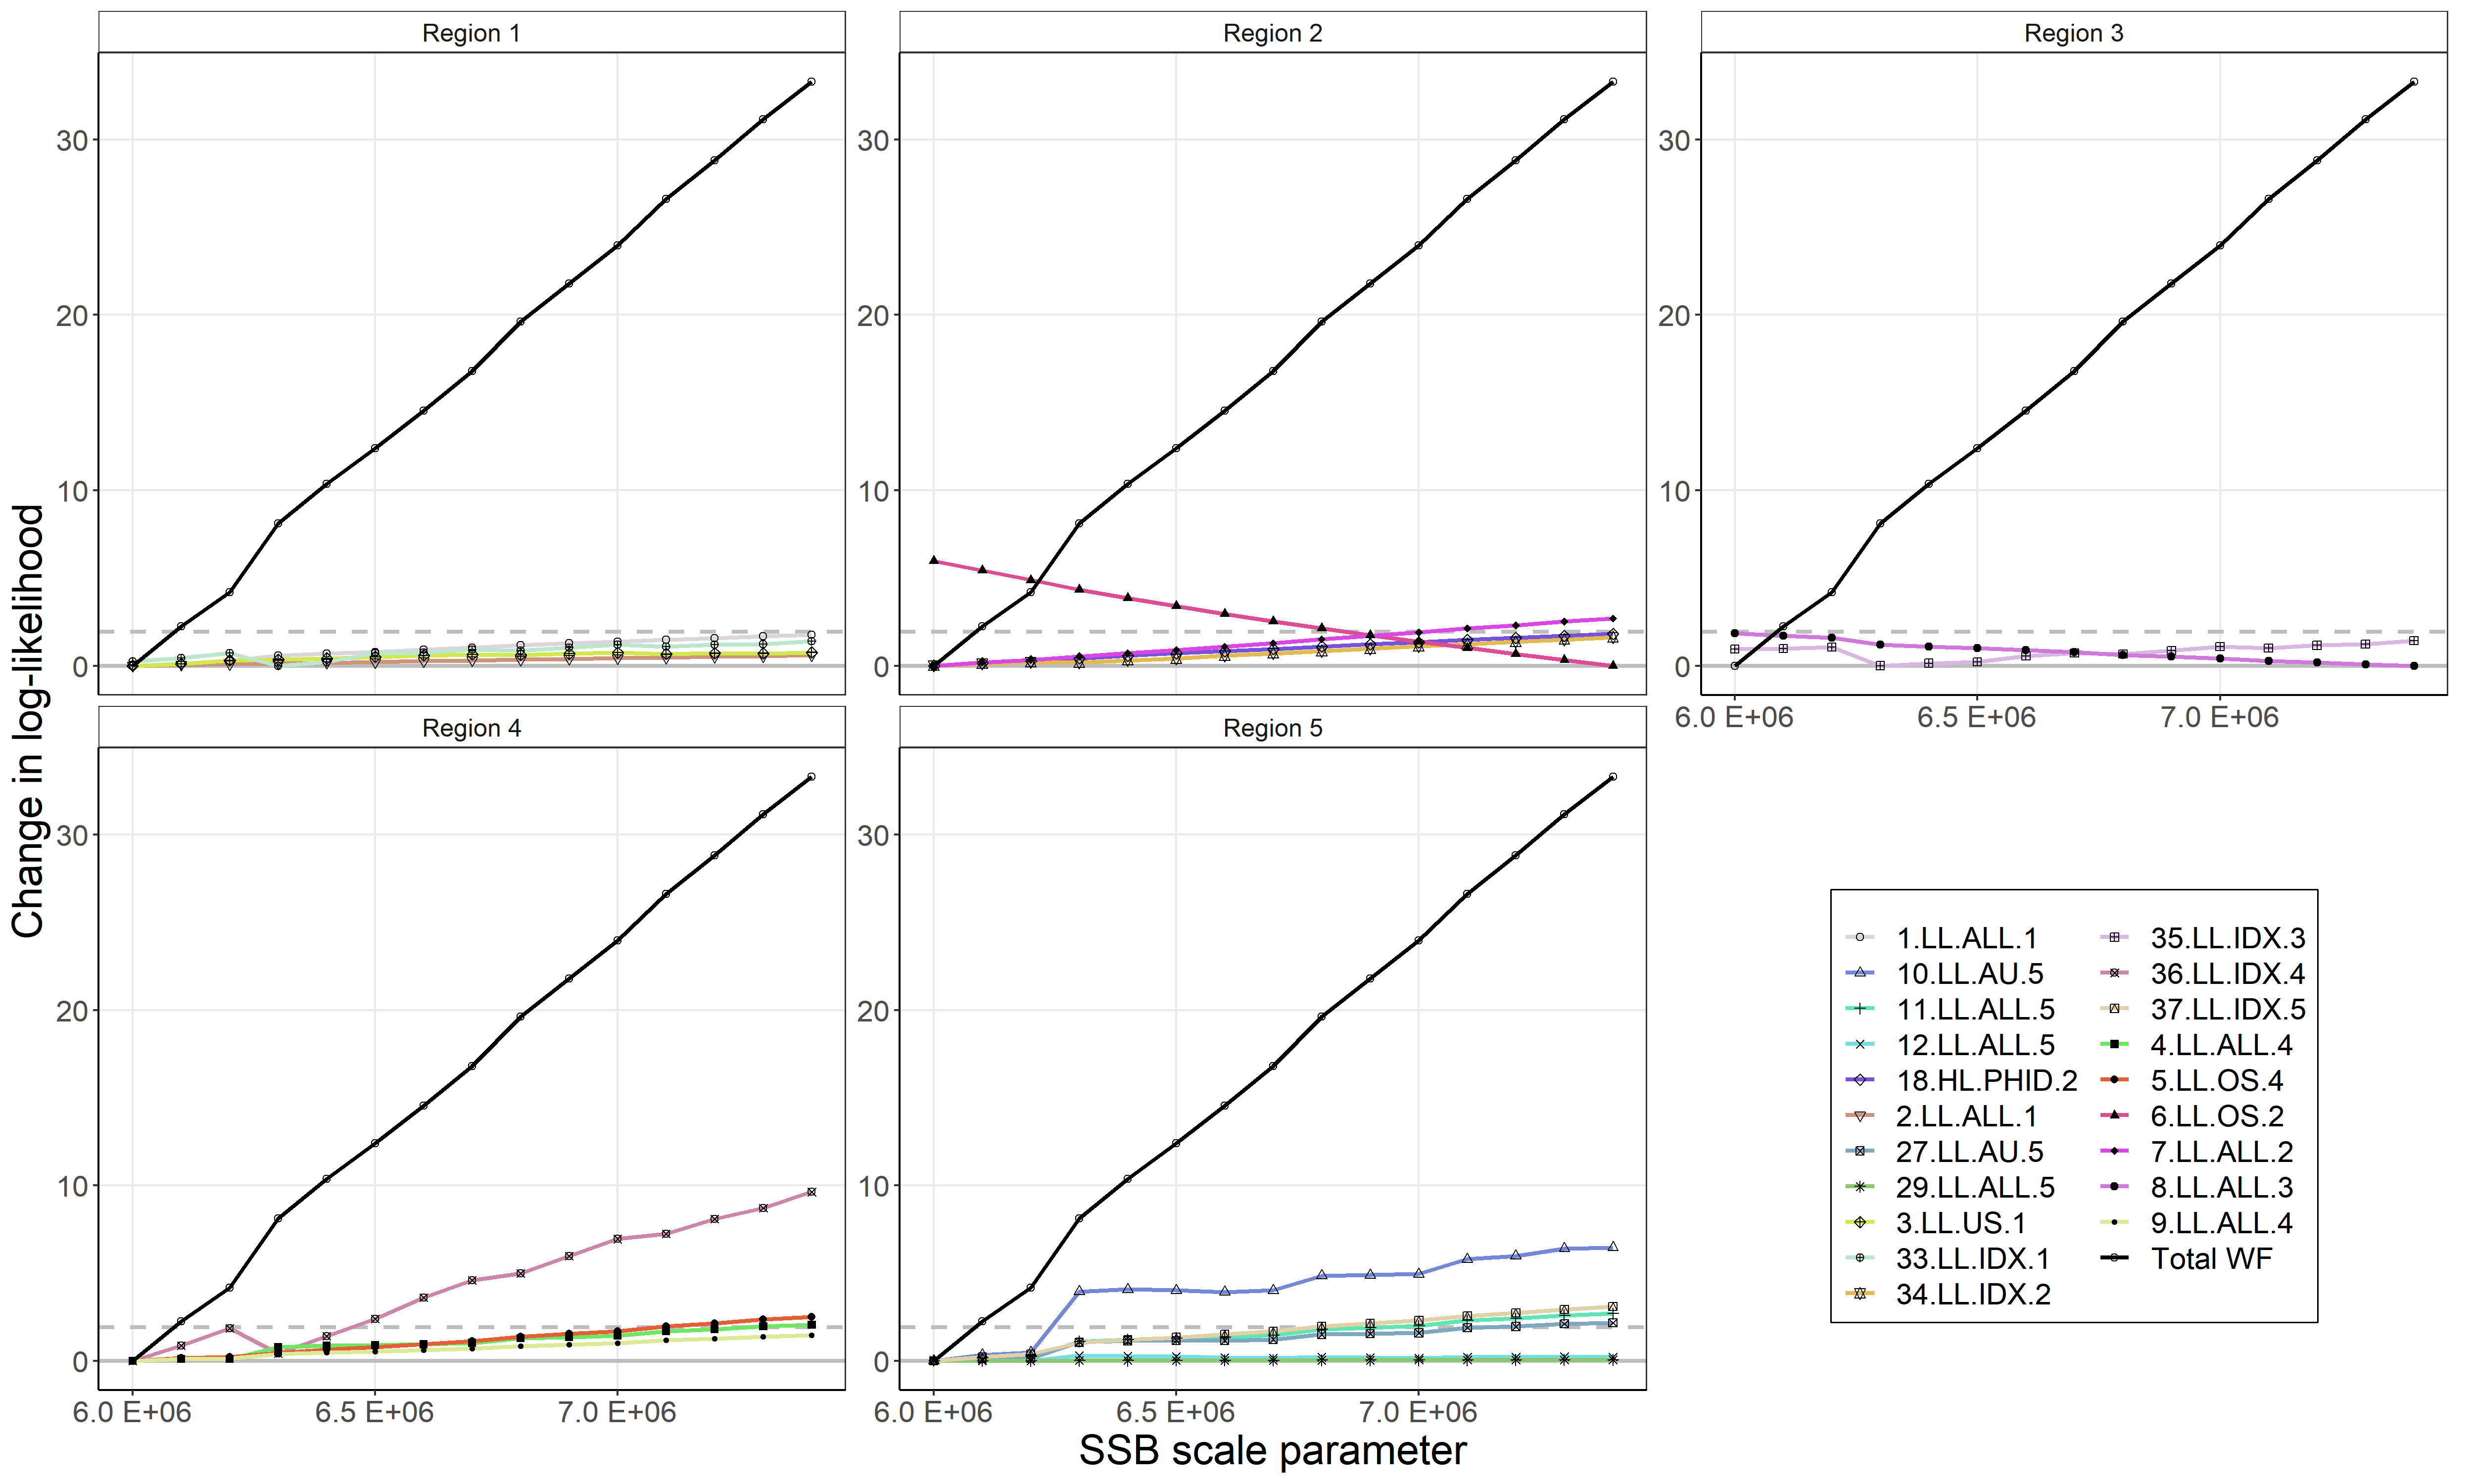
\includegraphics[width=0.9\textwidth]{likelihoodprofile_weight_narrow.png}\\[10mm]
  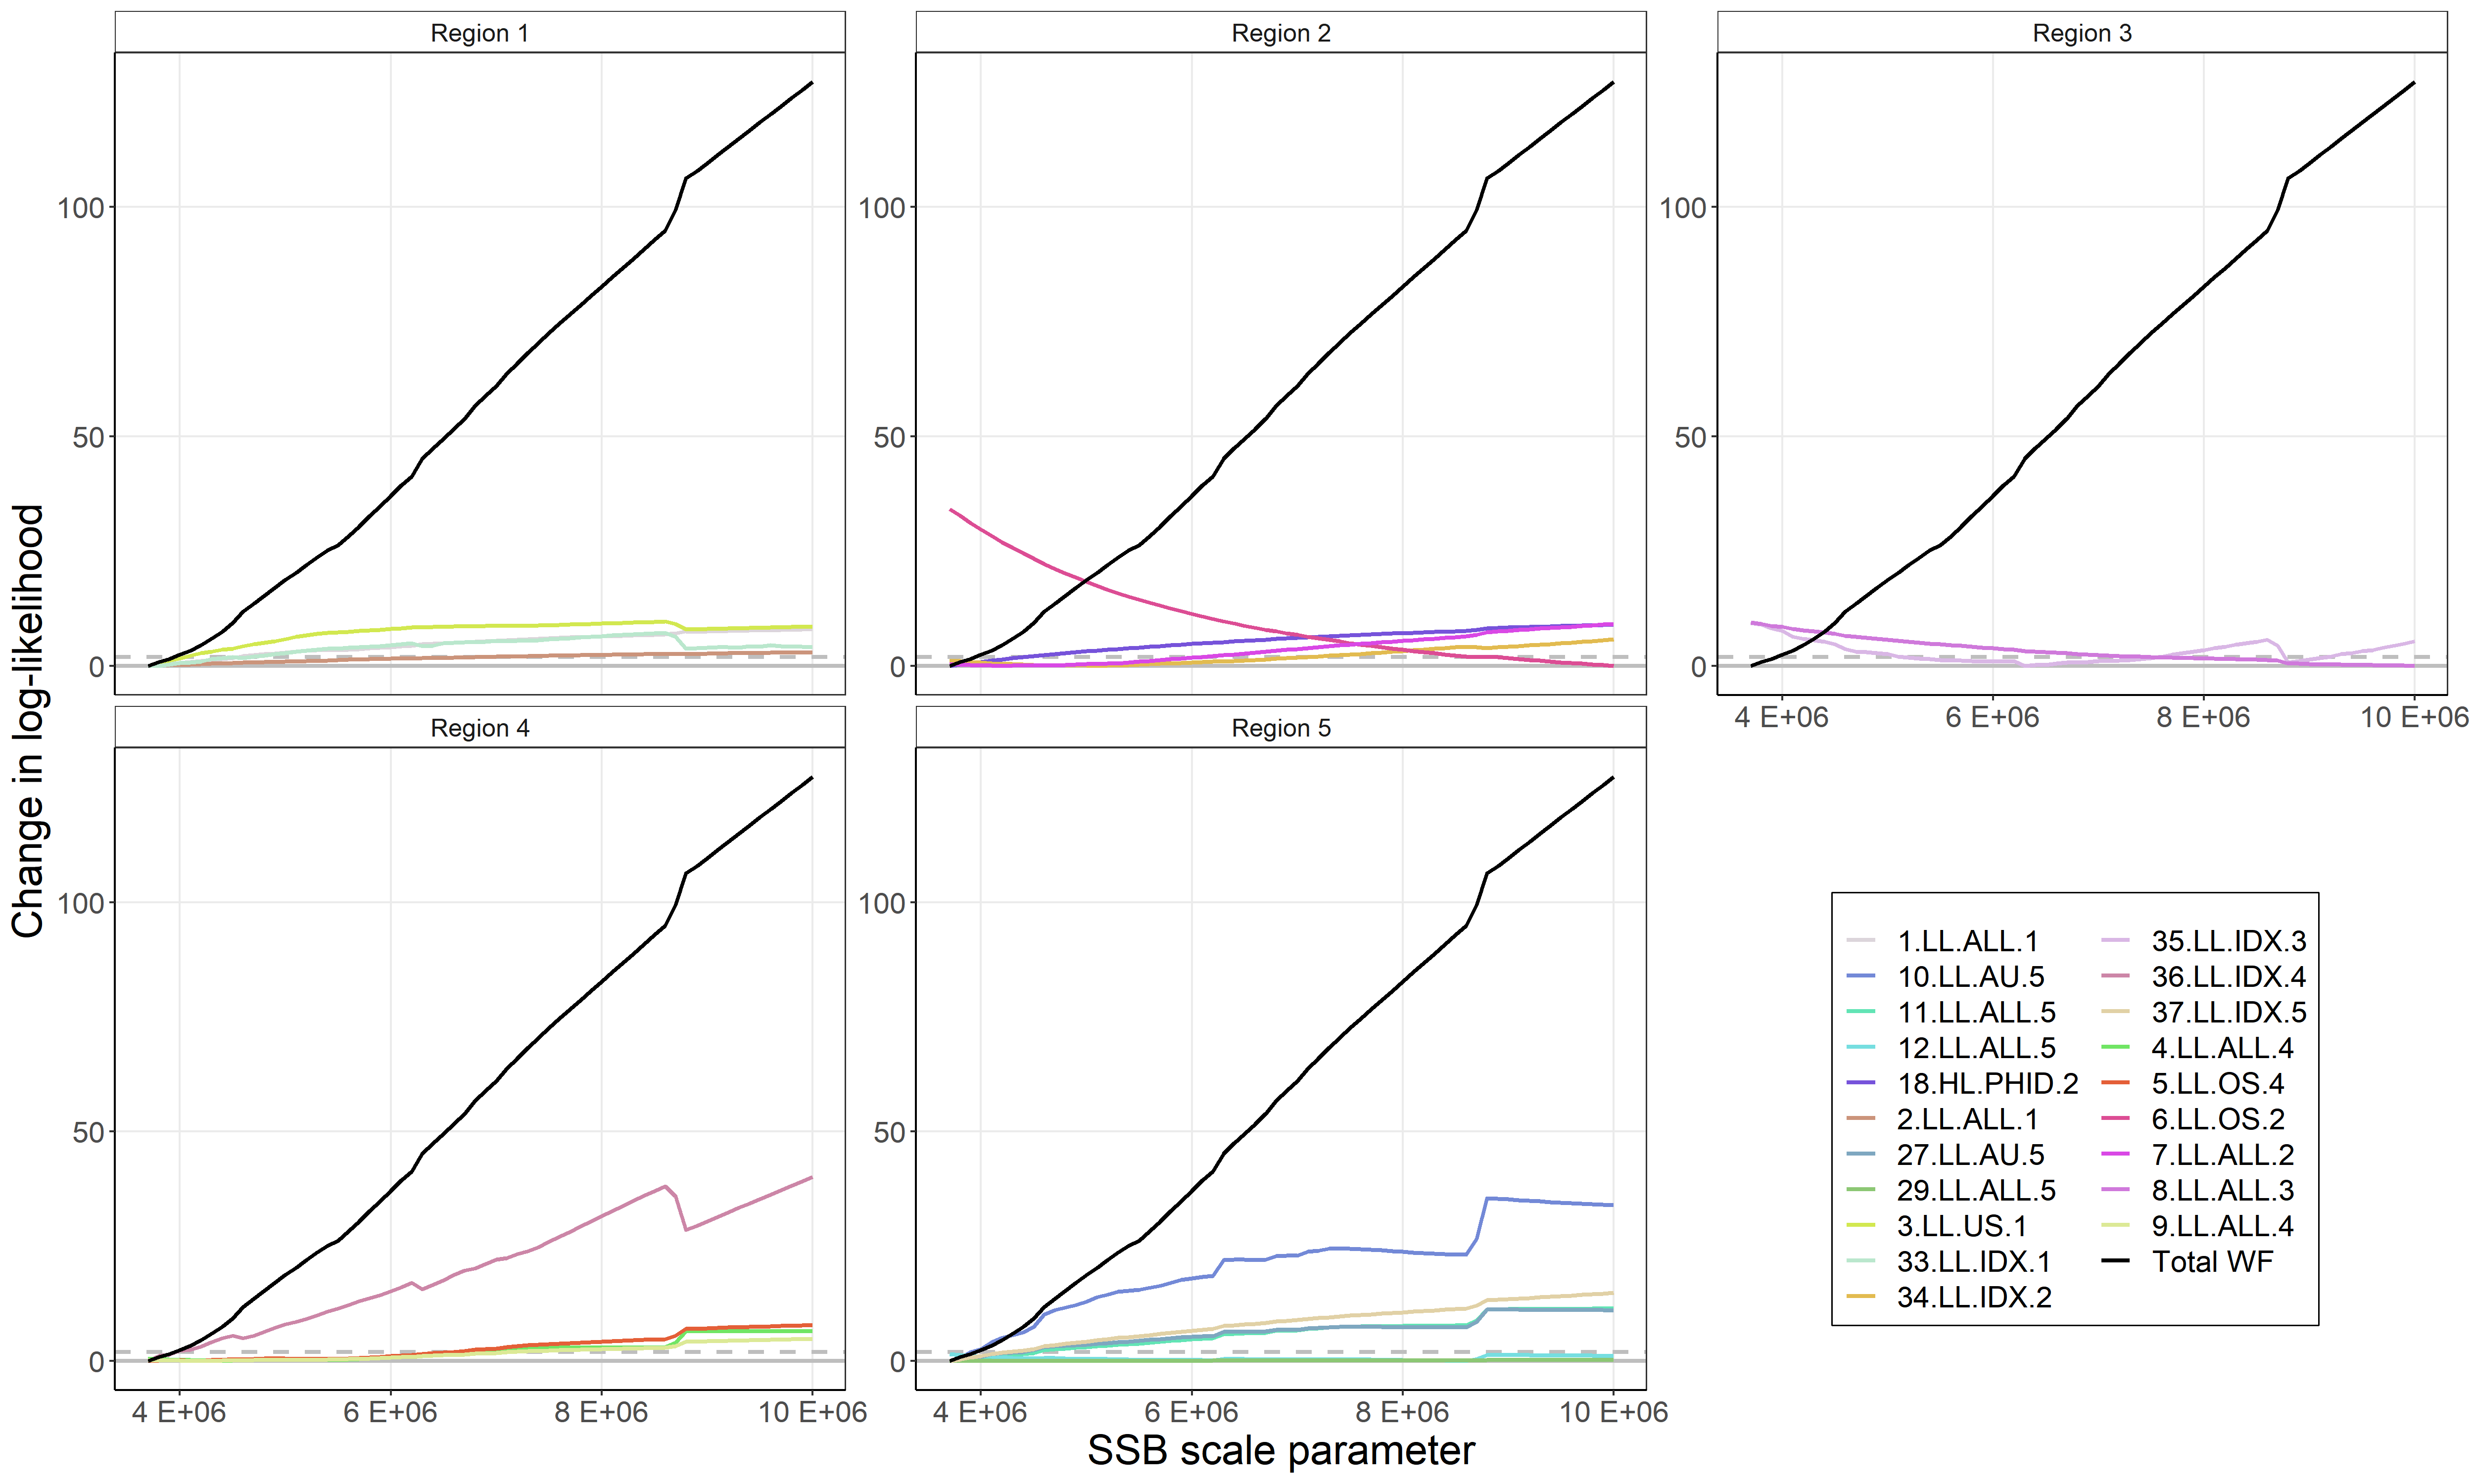
\includegraphics[width=0.9\textwidth]{likelihoodprofile_weight_wide.png}
  \caption{Profiles of the total log-likelihood with respect to average total biomass in million mt across a range of fixed values for the weight composition data by fishery and regions, the black line indicates the total weight composition likelihood. The top plot shows a narrow window around the total maximum likelihood estimated value and the bottom plot shows a wider window. \label{fig:likelihood_profile_weight}}
\end{figure}

\begin{figure}[H]
  \centering
  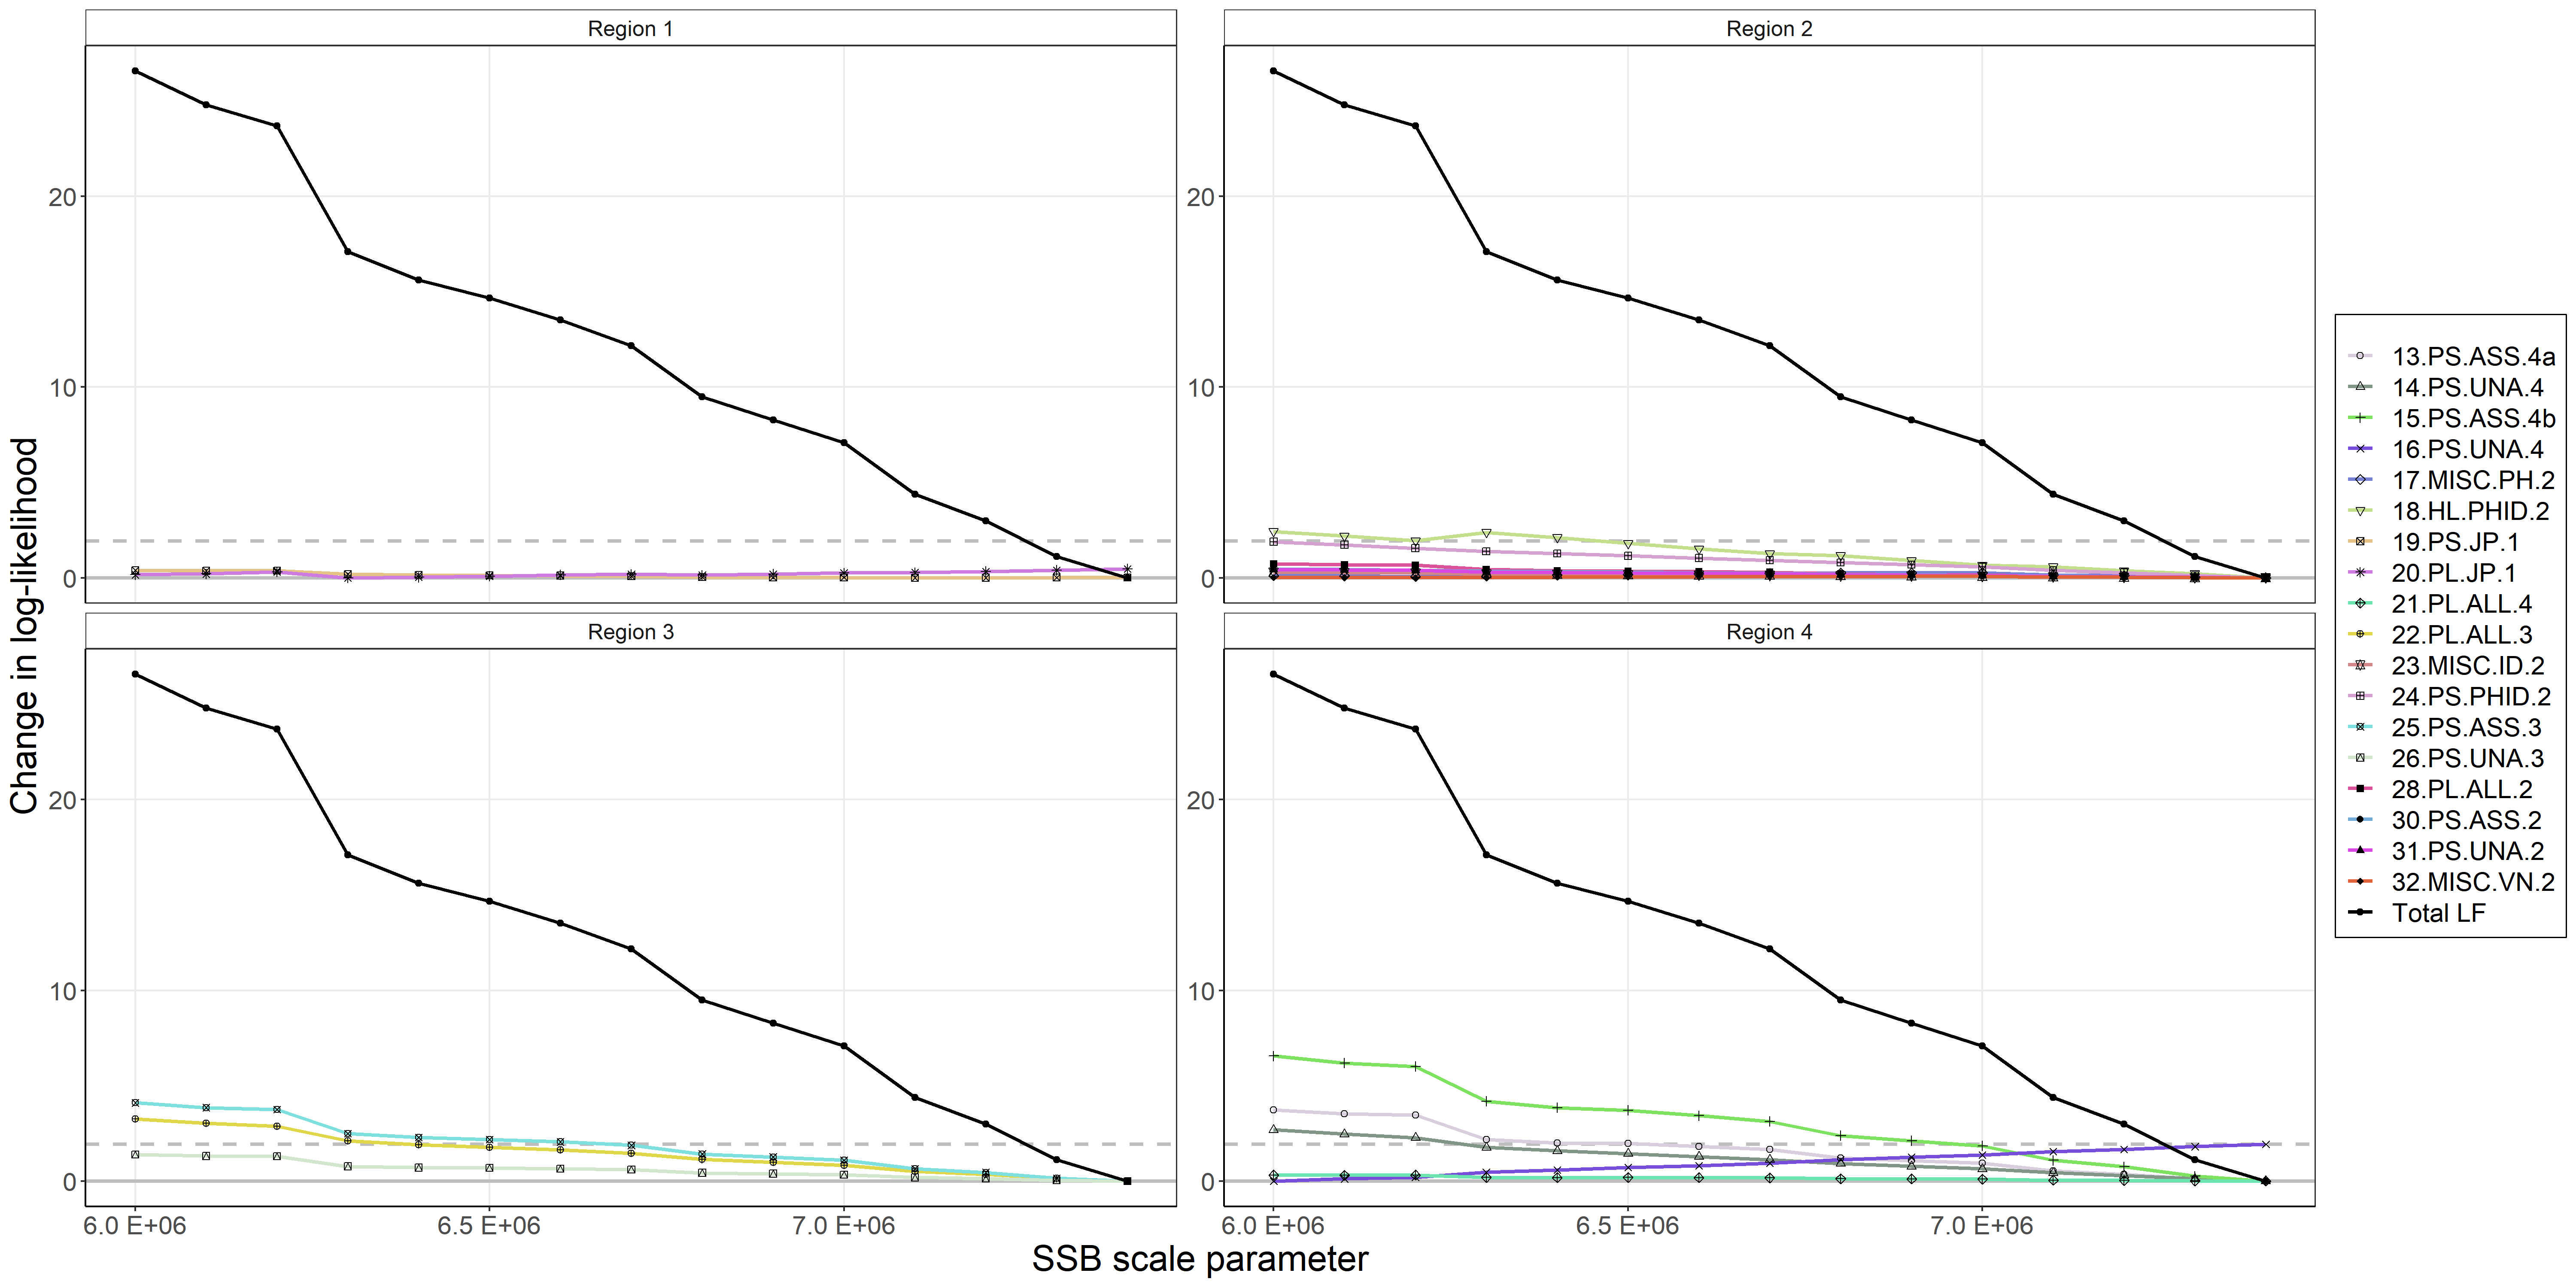
\includegraphics[width=\textwidth]{likelihoodprofile_length_narrow.png}\\[10mm]
  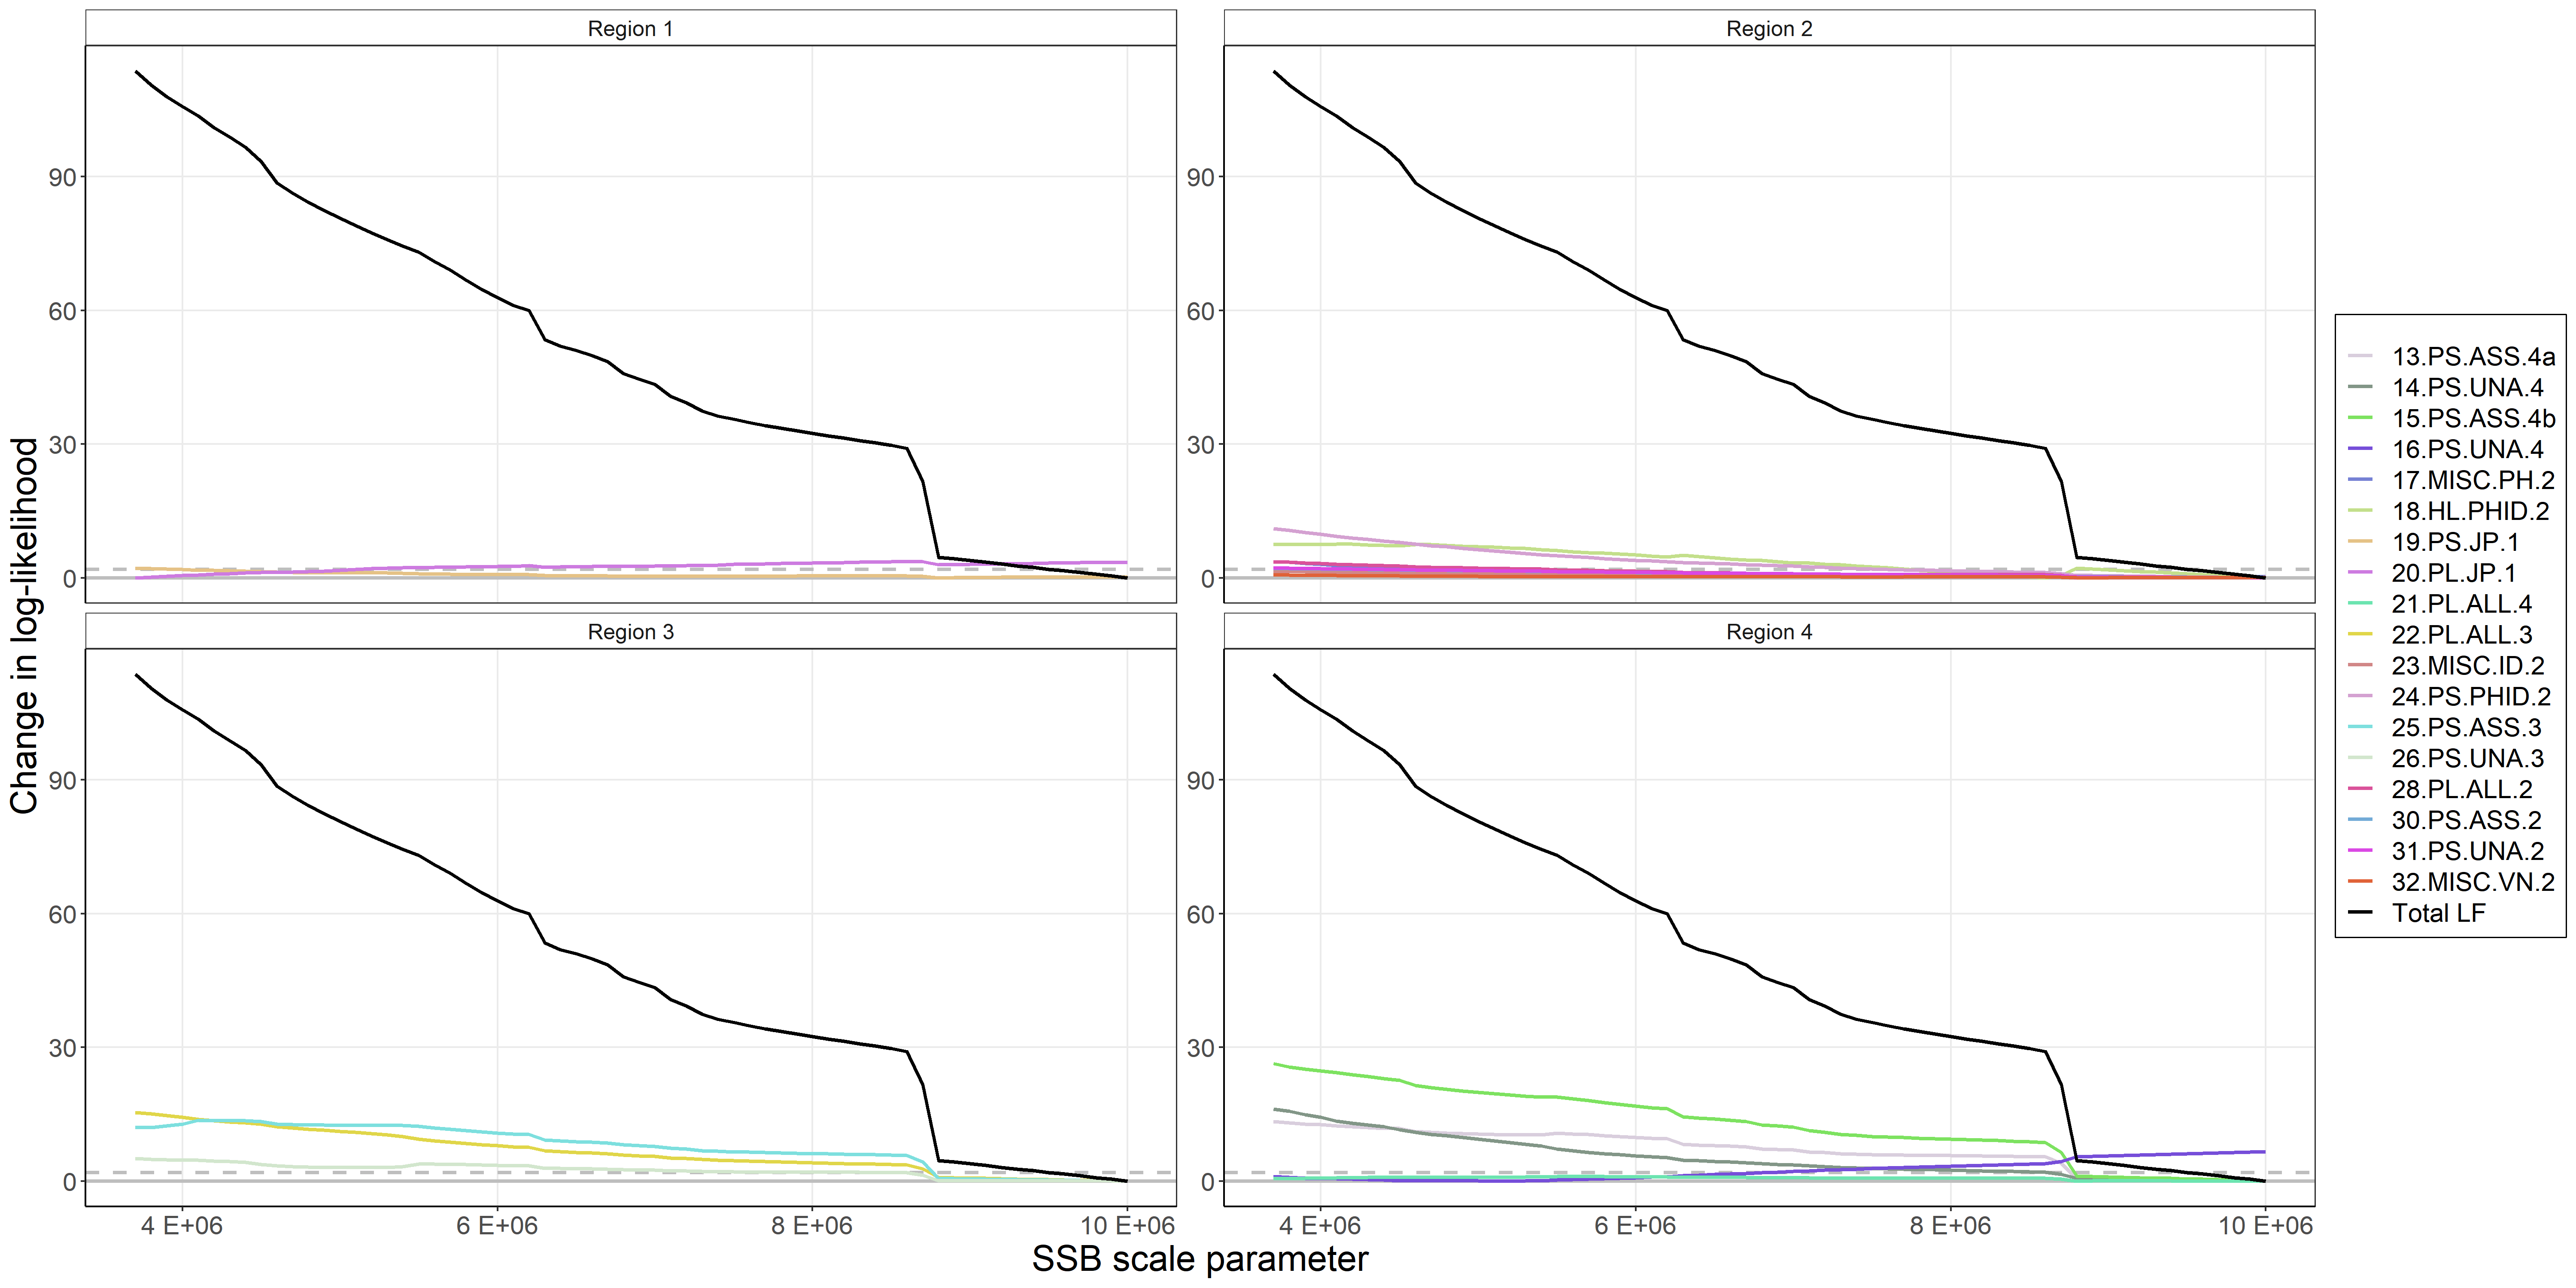
\includegraphics[width=\textwidth]{likelihoodprofile_length_wide.png}
  \caption{Profiles of the total log-likelihood with respect to average total biomass in million mt across a range of fixed values for the length composition data by fishery and regions, the black line indicates the total length composition likelihood. The top plot shows a narrow window around the total maximum likelihood estimated value and the bottom plot shows a wider window. \label{fig:likelihood_profile_length}}
\end{figure}

\clearpage

\subsection{Retrospective analyses}
\label{sec:retro_analysis}

Retrospective analysis involves rerunning the 2023 diagnostic model by consecutively removing successive years of data to estimate model bias. A series of 7 retrospective models were fitted starting with the full dataset (through 2021), followed by models with the retrospective removal of all input data for each year peel. Spawning potential and spawning depletion trajectories are shown in \autoref{fig:retrospectives}. Mohns rho is calculated for the retrospective models of spawning depletion.

Spawning potential and spawning depletion trajectories for each of these retrospective peels are shown in \autoref{fig:retrospectives}. Each peel produces estimates of spawning potential and spawning depletion with very similar dynamics to the diagnostic model. The value of Mohn's rho is 0.084 for the spawning depletion retrospectives, and $-0.101$ for spawning potential (\autoref{fig:retrospectives}). As a general rule of thumb, values of Mohn’s rho higher than 0.20 or lower than $-0.15$ are cause for concern in an assessment \citep{hurtado-ferro_looking_2015}. The values obtained for the 2023 yellowfin diagnostic model indicate that there is no strong concern for retrospective bias with the 2023 diagnostic model.

\begin{figure}[H]
  \centering
  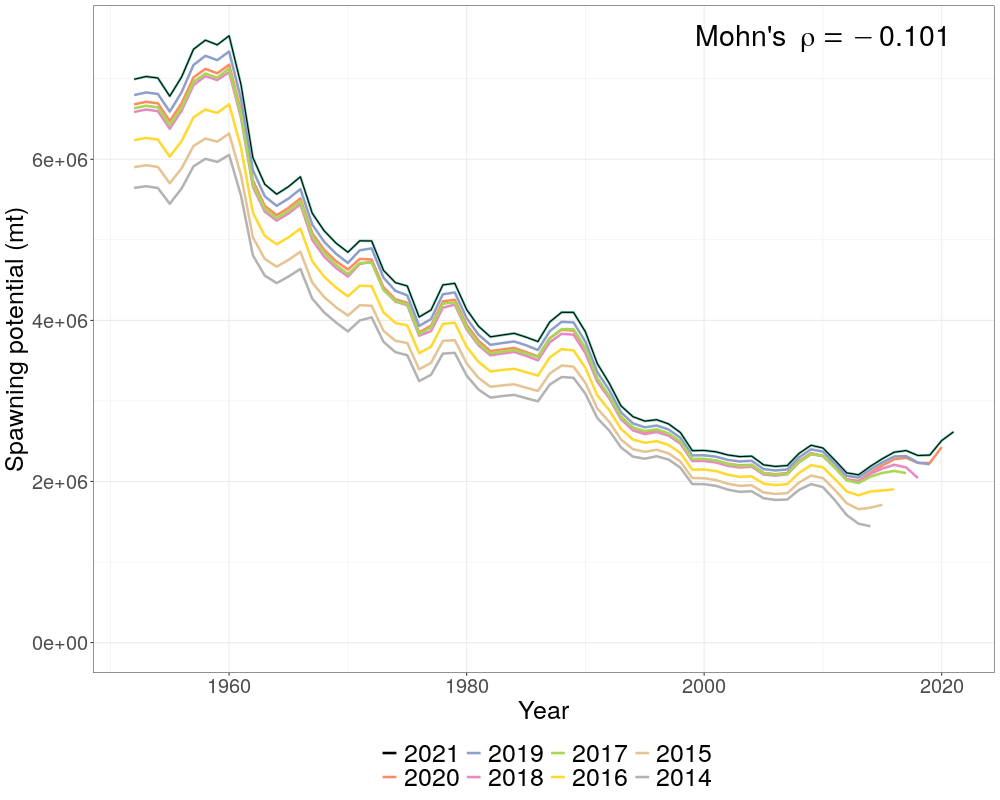
\includegraphics[width=0.7\textwidth]{retro_spawning_potential.png}\\[10mm]
  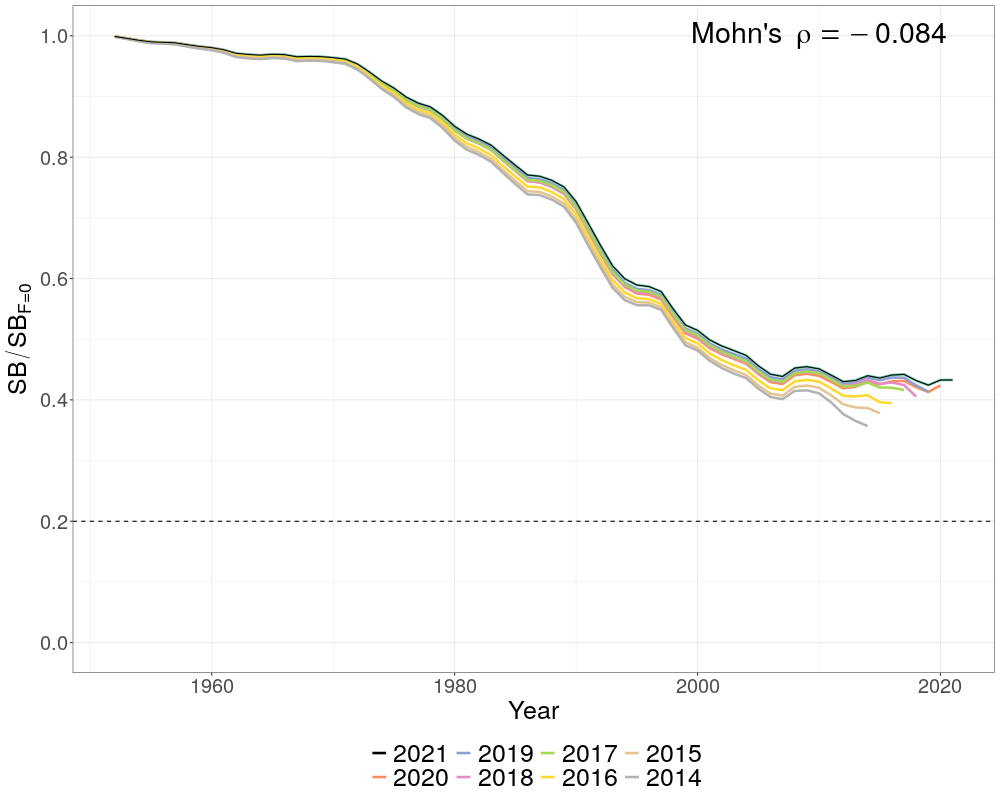
\includegraphics[width=0.7\textwidth]{retro_depletion.png}
  \caption{Estimated spawning potential (top) and spawning depletion (bottom) for the retrospective models. \label{fig:retrospectives}}
\end{figure}

\clearpage

\subsection{‘Status quo’ stochastic stock projections for WCPO yellowfin tuna}
\label{sec:projections}

These will be completed for the Tropical Tuna Measure meeting.

\newpage
\clearpage
\clearpage
